\documentclass[12pt,twoside]{article}
\title{M374M Homework 10 \\
  \normalsize{\S~4.2 \#3$^1$, 13$^2$ \S~4.3 \#2$^3$ab, 4} \\
  Revision: \input{revision}}
\author{Hershal Bhave (hb6279)}
\date{Due 2016--04--15}

\usepackage{homework-macros}
\tikzexternalize%

\begin{document}
\maketitle

\section{\S~4.2}
\subsection{3$^1$}
\subsubsection*{Problem}
Consider the functional
\begin{equation}
  \label{eq:4.2.3-problem}
  J(y)=\int_0^1(1+x){(y')}^2\dd{x}
\end{equation}
over the domain $\{y\in C^2[0,1]\;|\;y(0)=0,y(1)=1\}$. Show that $\delta
J(y_0,h)=0\;\forall h\in C^2$ and $h(0)=h(1)=0$, where $y_0(x)=\ln (1+x)/\ln2$.

\subsubsection*{Remarks}
Find first variation at $y_0$ for arbitrary $h$ as described, and show result
vanishes. The functional is $$J(y)=\int_0^1(1+x){(y')}^2\dd{x}.$$

\subsubsection*{Solution}
\begin{equation*}
  \begin{aligned}
    J(y_0+\epsilon h) &= \int_0^1(1+x){(y'(x))}^2\dd{x} \\
    \od{}{\epsilon} J(y_0+\epsilon h(x)) &= \od{}{\epsilon} \int_0^1(1+x){(y'(x))}^2\dd{x} \\
    &= \int_0^1 (1+x) (2h'(x)y_0'(x) + 2\epsilon {h'(x)}^2) \dd{x} \\
    {\left[ \od{}{\epsilon} J(y_0+\epsilon h(x)) \right]}_{\epsilon=0} &= \int_0^1 (1+x) (2h'(x)y_0'(x)) \dd{x} \\
    &= \int_0^1 \cancel{(1+x)} (2h'(x)\frac{1}{\cancel{(1+x)}\ln2}) \dd{x} \\
    \delta J(y_0,h) &= \frac{2}{\ln2}\int_0^1 h'(x) \dd{x} \\
    &= \frac{2}{\ln2}{\left[ h(x) \right]}_{x=0}^{x=1} \\
    &= \frac{2}{\ln2}(h(1)-h(0)) \\
  \end{aligned}
\end{equation*}

\begin{equation*}
  \boxed{\implies \delta J(y_0,h) = 0.}
\end{equation*}

\subsection{13$^2$}
\subsubsection*{Problem}
The second variation of a functional $J:A\rightarrow\mathbb{R}$ at $y_0\in A$ in
the direction $h$ is defined by
\begin{equation}
  \label{eq:4.2.13-problem}
  \delta^2J(y_0,h)\equiv \left[\od[2]{}{\epsilon} J(y_0+\epsilon h)\right]_{\epsilon=0}.
\end{equation}
Find the second variation of the functional
\begin{equation}
  \label{eq:4.2.13-problem-second-variation}
  J(y)=\int_0^1(xy'^2+y\sin y')\dd{x},
\end{equation}
where $y\in C^2[0,1]$.

\subsubsection*{Remarks}
For arbitrary $y$ and $h$ consider $J(y+\epsilon h)$. Find an expression for the
second variation $${\left[\od[2]{}{\epsilon} J(y+\epsilon h)\right]}_{\epsilon=0}$$

\subsubsection*{Solution}
Since the derive and integrate operators are linear, we may rearrange the
problem to make the task easier.
\begin{equation*}
  \begin{aligned}
    {\left[\od[2]{}{\epsilon} J(y+\epsilon h)\right]}_{\epsilon=0}
    &= {\left[\od[2]{}{\epsilon} \int_0^1(x{(y'+\epsilon h')}^2+(y+\epsilon h)\sin(y'+\epsilon h'))\dd{x} \right]}_{\epsilon=0} \\
    &= \int_0^1{\left[\od[2]{}{\epsilon} (x{(y'+\epsilon h')}^2+(y+\epsilon h)\sin(y'+\epsilon h'))\right]}_{\epsilon=0}\dd{x} \\
  \end{aligned}
\end{equation*}
Expand
\begin{equation*}
  \int_0^1{\left[\od[2]{}{\epsilon}
      2 x \epsilon h' y_0'+x \epsilon ^2 \left(h'\right)^2+h \epsilon \sin
      \left(\epsilon h'+y_0'\right)+y_0 \sin \left(\epsilon h'+y_0'\right)+x
      \left(y_0'\right){}^2
    \right]}_{\epsilon=0}\dd{x}
\end{equation*}
Derive
\begin{equation*}
  \int_0^1{\left[
      2 x \left(h'\right)^2-h \epsilon \left(h'\right)^2 \sin \left(\epsilon
        h'+y_0'\right)-y_0 \left(h'\right)^2 \sin \left(\epsilon h'+y_0'\right)+2 h h'
      \cos \left(\epsilon h'+y_0'\right)
    \right]}_{\epsilon=0}\dd{x}
\end{equation*}
Evaluate $\epsilon=0$
\begin{equation*}
  \boxed{\int_0^1
      2 x \left(h'\right)^2-y_0 \left(h'\right)^2 \sin \left(y_0'\right)+2 h h'
      \cos \left(y_0'\right)
    \dd{x}}
\end{equation*}

\section{\S~4.3}
\subsection{2$^3$a}
\subsubsection*{Problem}
Find extremals for
\begin{equation}
  \label{eq:4.3.2a-problem}
  \int_a^b \frac{{(y')}^2}{x^3}\dd{x}
\end{equation}

\subsubsection*{Remarks}
Assume $[a,b]=[1,2]$ and $y(1)=0$ and $y(2)=1$.

\subsubsection*{Solution}
Let
\begin{align*}
  L_y &= 0 \\
  L_{y'} &= \frac{2y'(x)}{x^3} \\
\end{align*}
so that
\begin{align*}
  L_y - \od{}{x} L_{y'} &= 0, \\
  -2 \od{}{x} y'(x) x^3 &= 0, \\
  -2\left[ y''(x) x^{-3}-3x^{-4}y'(x) \right] &= 0.
\end{align*}
Solving this ODE results in
\begin{equation*}
  y(x)=c_1x^4+c_2.
\end{equation*}
Invoking the initial conditions resolves the constants.
\begin{equation*}
  \boxed{\frac{1}{15}(x^4-1)}
\end{equation*}

\subsection{2$^3$b}
\subsubsection*{Problem}
Find extremals for
\begin{equation}
  \label{eq:4.3.2b-problem}
  \int_a^b(y^2+{(y')}^2 + 2ye^x)\dd{x}.
\end{equation}

\subsubsection*{Remarks}
Assume $[a,b]=[1,2]$ and $y(1)=0$ and $y(2)=1$.
\subsubsection*{Solution}
Let
\begin{align*}
  L_y &= 2y(x)+2e^x \\
  L{y'} &= 2y'(x)
\end{align*}
so that
\begin{align*}
  L_y - \od{}{x} L_{y'} &= 0, \\
  2y(x) + 2e^x - 2y''(x) &= 0. \\
\end{align*}
Solving this ODE results in
\begin{equation*}
  y(x) = c_1 e^x + c_2 e^{-x} + \frac{x e^x}{2}.
\end{equation*}
Invoking the initial conditions resolves the constants.
\begin{equation*}
  \boxed{y(x) = \frac{e^x x}{2}+3.11627 e^{-x}-0.921741 e^x}
\end{equation*}

\subsection{4}
\subsubsection*{Problem}
Find an extremal for all
\begin{equation}
  \label{eq:4.3.4-problem}
  J(y) = \int_1^2\frac{\sqrt{1+{(y')}^2}}{x}\dd{x},\quad y(1)=0,\quad y(2)=1.
\end{equation}
\subsubsection*{Solution}
Let
\begin{align*}
  L_y &= 0 \\
  L_{y'} &= \frac{y'(x)}{x\sqrt{1+{(y'(x))}^2}} \\
\end{align*}
We may use the short form of the Euler-Lagrange equation to solve this system.
\begin{align*}
  c &= L_{y'}(x,y') \\
  c &= \frac{y'(x)}{x\sqrt{1+{(y'(x))}^2}} \\
  y'(x) &= cx\sqrt{1+{(y'(x))}^2} \\
  {(y'(x))}^2 &= c^2x^2 + c^2 x^2 {(y'(x))}^2 \\
  {(y'(x))}^2(1-c^2x^2) &= c^2x^2 \\
  {(y'(x))}^2 &= \frac{c^2x^2}{1-c^2x^2} \\
  y'(x) &= \frac{cx}{\sqrt{1-c^2x^2}} \\
  \implies y(x) &= \frac{\sqrt{1-c_1^2x^2}}{c_1}+c_2 \\
\end{align*}
Invoking the initial conditions resolves the constants
\begin{equation*}
  \boxed{y(x) = 2-\sqrt{5-x^2}}
\end{equation*}
\section{Minilab}
When stretched between two symmetrically placed rings, a thin soap film will
form a curved surface of revolution. If we denote the profile curve by $y(x)$
where $x\in[-L,L]$, then the surface area is given by
\begin{equation}
  \label{eq:minilab-surface-area}
  A(y)=\int_{-L}^L 2\pi y(x) \sqrt{1 + {\left[ y'(x) \right]}^2}\dd{x}.
\end{equation}
The specific shape adopted by the film can be described as that which minimizes
the functional $A(y)$ in a given function space. Here we find candidates for
local minimizers in the $C^2$-norm in the space $\mathcal{V}=\{y\in
C^2[-L,L]\;|\;y(-L)=\alpha,\;y(L)=\beta,\;y(x)>0\}$. For simplicity, we assume
$\alpha=\beta>0$.

\begin{enumerate}[(a)]
\item
\subsubsection*{Problem}
After a change of variable $x\rightarrow x/L$ and $y\rightarrow y/L$, show that
any local minimizer $y_*\in \mathcal{V}$ must satisfy the following
boundary-value problem, where $\gamma=\alpha/L$:
\begin{equation}
  \label{eq:minilab.a-problem}
  yy''-{(y')}^2=1,\quad -1\le x\le1. \qquad y(-1)=\gamma,\quad y(1)=\gamma.
\end{equation}

\subsubsection*{Solution}
Let
$$L = 2\pi y(x) \sqrt{1 + {\left[ y'(x) \right]}^2}.$$
Then
\begin{align*}
  L_y(x,y,y') &= 2\pi {(1+{(y'(x))}^2)}^{1/2} \\
  L_{y'}(x,y,y') &= \frac{2\pi y(x) y'(x)}{{(1+{(y'(x))}^2)}^{1/2}}. \\
\end{align*}
So that the Euler-Lagrange equation for this system is
\begin{align*}
  0 &= L_y(x,y,y') - \od{}{x}L_{y'}(x,y,y') \\
  \implies 0 &= 2\pi {(1+{(y'(x))}^2)}^{1/2} - \od{}{x} \frac{2\pi y(x) y'(x)}{{(1+{(y'(x))}^2)}^{-1/2}} \\
  2\pi {(1+{(y'(x))}^2)}^{1/2} &= \od{}{x} \frac{2\pi y(x) y'(x)}{{(1+{(y'(x))}^2)}^{-1/2}} \\
  \frac{(1+{(y'(x))}^2)}{y(x)} &= \od{}{x} y'(x) \\
  \frac{(1+{(y'(x))}^2)}{y(x)} &= y''(x) \\
  1+{(y'(x))}^2 &= y(x) y''(x) \\
  \implies y(x) y''(x) - {(y'(x))}^2 &= 1 \\
\end{align*}
Furthermore, the boundary conditions adapt to the scaling:
\begin{align*}
  y(-L), &= \alpha &\quad\implies y(-1) &= \alpha/L, &\quad\implies y(-1) &= \gamma \\
  y(L), &= \alpha &\quad\implies y(1) &= \beta/L=\alpha/L, &\quad\implies y(1) &= \gamma \\
\end{align*}

\item
\subsubsection*{Problem}
Consider the smooth function
\begin{equation}
  \label{eq:minilab.b-problem-smooth}
  y_*(x)=\frac{1}{c}\cosh(cx+d),
\end{equation}
where $c>0$ and $d$ are arbitrary constants. Show that $y_*$ satisfies the
differential equation. Moreover, show that $y_*$ will satisfy the boundary
conditions and hence will be in the space $\mathcal{V}$ only if $d=0$ and $c>0$
satisfies
\begin{equation}
  \label{eq:minilab.b.problem-satisfy}
  \cosh(c) = \gamma c.
\end{equation}

\subsubsection*{Solution}
Given
\begin{align*}
  y_*(x) &= \frac{1}{c}\cosh(cx+d) \\
  y_*'(x) &= \sinh(cx+d) \\
  y_*''(x) &= c\cosh(cx+d), \\
\end{align*}
then \cref{eq:minilab.a-problem} becomes
\begin{equation}
  \label{eq:minilab.b-identity}
  \cosh^2(cx+d) - \sinh^2(cx+d) = 1.
\end{equation}
This is a trigonometric identity, so it is always true. Furthermore, the only
way \cref{eq:minilab.b-identity} can satisfy the boundary conditions is when
$d=0$ since $\cosh$ is symmetric across the $y$ axis, and when $c>0$ since
$\cosh$ is never negative.

\item
\subsubsection*{Problem}
Show that \cref{eq:minilab.b.problem-satisfy} has two solutions for $c$ if
$\gamma > \gamma_{\#}$, one solution if $\gamma = \gamma_{\#}$, and no solution
if $0<\gamma<\gamma_{\#}$, where $\gamma_{\#}$ is an appropriate constant which
you should find. Hence we have two, one, or no candidates for a local minimizer
$y_*\in\mathcal{V}$ depending on the value of $\gamma$.

\subsubsection*{Solution}
Reference \cref{fig:minilab.c-gamma-intercept}. Notice that there are two
intersections of $y(c)$ with the $\gamma$-line when $\gamma>\gamma_{\#}$, one
intersection when $y(c)$ is tangent to $\gamma_{\#}$, and no intersections when
$\gamma<\gamma_{\#}$. We found the intersection point to be approximately $(1.2,
1.5088)$. Hence there are two, one, or zero candidates for a local minimizer
$y_*\in\mathcal{V}$ depending on $\gamma$.
\begin{figure}
  \centering
  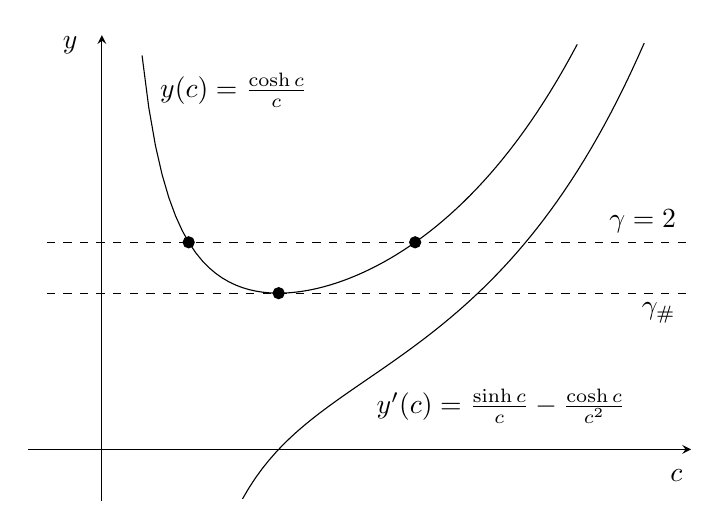
\begin{tikzpicture}
    \begin{axis}[width=10cm, height=7.5cm,
      domain=-.5:4,
      xmin=-.5, xmax=4, restrict x to domain=-.5:4,
      ymin=-.5, ymax=4, restrict y to domain=-.5:4,
      view={0}{90}, xlabel=$c$, ylabel=$y$,
      axis lines=middle, xtick=\empty, ytick=\empty,
      x label style={at={(axis cs:3.9,-0.1)},anchor=north},
      y label style={at={(axis cs:-0.1,3.9)},anchor=east}]

      \addplot[domain=-.5:4,samples=100] {cosh(x)/x} node[above right,pos=0.1]{$y(c)=\frac{\cosh c}{c}$};
      \addplot[domain=-.5:4,samples=100] {sinh(x)/x-cosh(x)/x^2} node[below right,pos=0.275]
      {$y'(c)=\frac{\sinh c}{c}-\frac{\cosh c}{c^2}$};
      \addplot[dashed,domain=-1:4] {1.5088} node[below,pos=0.95]{$\gamma_{\#}$};
      \addplot[only marks] coordinates {(1.2,1.5088)};
      \addplot[dashed,domain=-1:4] {2} node[above,pos=0.925]{$\gamma=2$};
      \addplot[only marks] coordinates {(.589387,2) (2.1268, 2)};
    \end{axis}
  \end{tikzpicture}
  \caption{$\gamma_{\#}$ intercept}
  \label{fig:minilab.c-gamma-intercept}
\end{figure}

\item
\subsubsection*{Problem}
In the case when $\gamma > \gamma_{\#}$ and there are two candidate curves
$y_*$, it can be shown that the candidate with the smaller $c$ is indeed a local
minimizer whereas the other is not. Find an make plots of these curves on
$[-1,1]$ for the case $\gamma=2$ and indicate which is the local minimizer. When
$\gamma\le\gamma_{\#}$, it can be shown that there are no local minimizers of
$A$ in $\mathcal{V}$; in this case, a surface of minimum area no longer has a
class $C^2$ profile graph. What do you think might happen to the soap film in
this case?

\subsubsection*{Solution}
Reference \cref{fig:minilab.c-gamma-intercept}. The smaller $c$ value is the
local minimizer. The profile seems to constrict as $\gamma$ decreases. Once
$\gamma=\gamma_{\#}$, a singularity occurs and the soap film splits into
bubbles.

\end{enumerate}

\end{document}
